%% fig_lefschetzgrid.tex   (generated by make_frontier.py; do not edit by hand)
%% The summands H^p(C,R^q) of an abelian scheme of relative dimension four over a curve, the operators of the proof, and the values for a Mumford family.
\documentclass[tikz,border=6pt]{standalone}
\usepackage{amsmath,amssymb}
\usetikzlibrary{arrows.meta,calc,decorations.pathreplacing,patterns}
%% palette.tex -- shared colour definitions for the figures
\definecolor{PInk}{RGB}{26,32,44}
\definecolor{PBlue}{RGB}{37,82,139}
\definecolor{PTeal}{RGB}{23,127,125}
\definecolor{POchre}{RGB}{193,138,44}
\definecolor{PClay}{RGB}{178,74,58}
\definecolor{PSlate}{RGB}{108,122,137}
\definecolor{PViolet}{RGB}{110,86,150}
\definecolor{WBlue}{RGB}{223,234,246}
\definecolor{WTeal}{RGB}{220,238,236}
\definecolor{WOchre}{RGB}{250,240,218}
\definecolor{WClay}{RGB}{247,229,224}
\definecolor{WSlate}{RGB}{238,241,244}
\definecolor{PMag}{RGB}{158,58,110}
\definecolor{PGrass}{RGB}{62,124,66}
\definecolor{PAmber}{RGB}{214,112,38}
\definecolor{PIndigo}{RGB}{58,64,140}
\definecolor{PRule}{RGB}{176,186,197}

%% shared macros so the standalone figures match the paper
\providecommand{\QQ}{\mathbb{Q}}
\providecommand{\ZZ}{\mathbb{Z}}
\providecommand{\RR}{\mathbb{R}}
\providecommand{\CC}{\mathbb{C}}
\providecommand{\PP}{\mathbb{P}}
\providecommand{\Kx}{K^{\times}}
\providecommand{\HW}{W}
\providecommand{\Nm}{\mathrm{N}}
\providecommand{\Hdg}{\mathrm{Hdg}}
\providecommand{\NS}{\mathrm{NS}}
\providecommand{\cA}{\mathcal{A}}
\providecommand{\cD}{\mathcal{D}}
\providecommand{\cF}{\mathcal{F}}
\providecommand{\cP}{\mathcal{P}}
\providecommand{\cO}{\mathcal{O}}
\providecommand{\cQ}{\mathcal{Q}}
\providecommand{\bbar}[1]{\overline{#1}}
\providecommand{\ch}{\operatorname{ch}}
\providecommand{\End}{\mathrm{End}}
\providecommand{\Ext}{\operatorname{Ext}}
\providecommand{\Supp}{\operatorname{Supp}}

\begin{document}
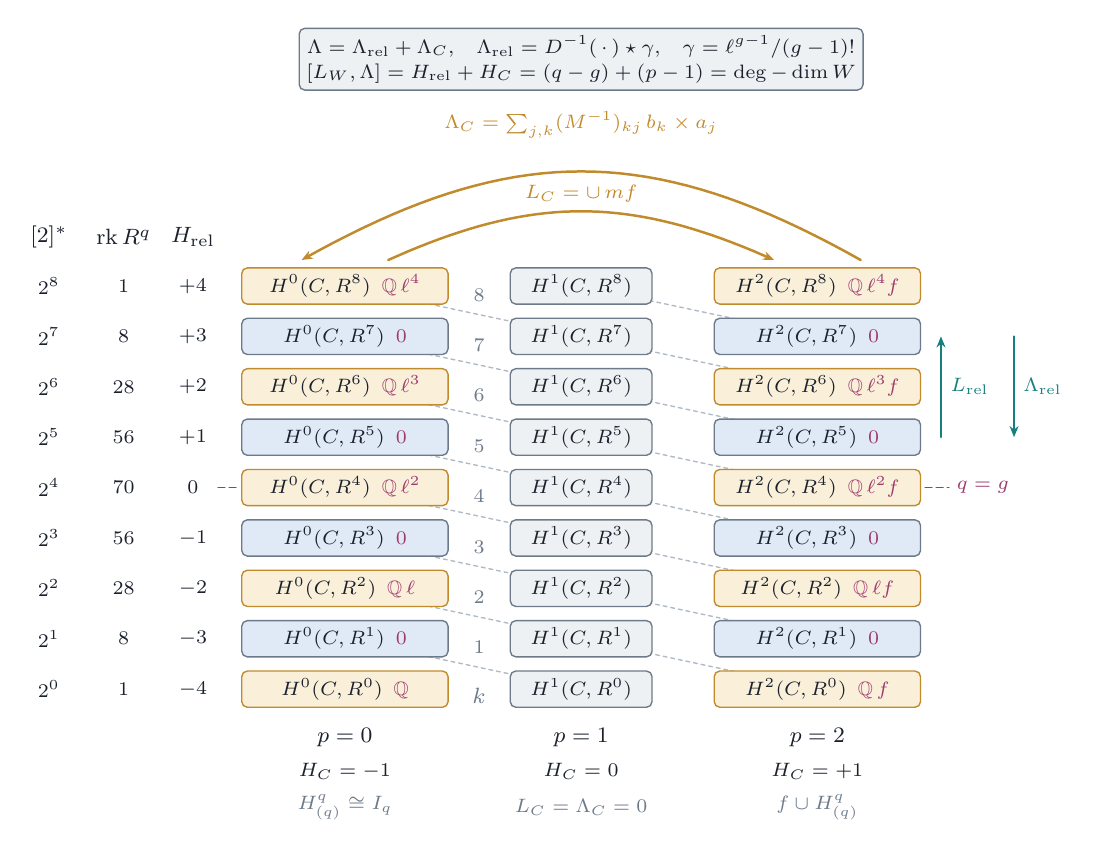
\begin{tikzpicture}[x=1cm,y=1cm,line join=round,line cap=round,
  font=\small,text=PInk]
  \draw[PRule,dash pattern=on 1.4pt off 1.4pt,line width=0.50pt] (0.000,0.640) -- (3.000,0.000);
  \draw[PRule,dash pattern=on 1.4pt off 1.4pt,line width=0.50pt] (0.000,1.280) -- (3.000,0.640) -- (6.000,0.000);
  \draw[PRule,dash pattern=on 1.4pt off 1.4pt,line width=0.50pt] (0.000,1.920) -- (3.000,1.280) -- (6.000,0.640);
  \draw[PRule,dash pattern=on 1.4pt off 1.4pt,line width=0.50pt] (0.000,2.560) -- (3.000,1.920) -- (6.000,1.280);
  \draw[PRule,dash pattern=on 1.4pt off 1.4pt,line width=0.50pt] (0.000,3.200) -- (3.000,2.560) -- (6.000,1.920);
  \draw[PRule,dash pattern=on 1.4pt off 1.4pt,line width=0.50pt] (0.000,3.840) -- (3.000,3.200) -- (6.000,2.560);
  \draw[PRule,dash pattern=on 1.4pt off 1.4pt,line width=0.50pt] (0.000,4.480) -- (3.000,3.840) -- (6.000,3.200);
  \draw[PRule,dash pattern=on 1.4pt off 1.4pt,line width=0.50pt] (0.000,5.120) -- (3.000,4.480) -- (6.000,3.840);
  \draw[PRule,dash pattern=on 1.4pt off 1.4pt,line width=0.50pt] (3.000,5.120) -- (6.000,4.480);
  \node[text=PSlate,inner sep=1pt,align=center,font=\scriptsize] at (1.705,0.526) {$1$};
  \node[text=PSlate,inner sep=1pt,align=center,font=\scriptsize] at (1.705,1.166) {$2$};
  \node[text=PSlate,inner sep=1pt,align=center,font=\scriptsize] at (1.705,1.806) {$3$};
  \node[text=PSlate,inner sep=1pt,align=center,font=\scriptsize] at (1.705,2.446) {$4$};
  \node[text=PSlate,inner sep=1pt,align=center,font=\scriptsize] at (1.705,3.086) {$5$};
  \node[text=PSlate,inner sep=1pt,align=center,font=\scriptsize] at (1.705,3.726) {$6$};
  \node[text=PSlate,inner sep=1pt,align=center,font=\scriptsize] at (1.705,4.366) {$7$};
  \node[text=PSlate,inner sep=1pt,align=center,font=\scriptsize] at (1.705,5.006) {$8$};
  \node[text=PSlate,inner sep=1pt,align=center,font=\footnotesize] at (1.705,-0.080) {$k$};
  \node[draw=POchre,fill=WOchre,rounded corners=2pt,inner sep=1pt,line width=0.50pt,align=center,font=\scriptsize,minimum width=2.62cm,minimum height=0.46cm] at (0.000,0.000) {$H^{0}(C,R^{0})$\enspace\textcolor{PMag}{$\mathbb{Q}$}};
  \node[draw=PSlate,fill=WBlue,rounded corners=2pt,inner sep=1pt,line width=0.50pt,align=center,font=\scriptsize,minimum width=2.62cm,minimum height=0.46cm] at (0.000,0.640) {$H^{0}(C,R^{1})$\enspace\textcolor{PMag}{$0$}};
  \node[draw=POchre,fill=WOchre,rounded corners=2pt,inner sep=1pt,line width=0.50pt,align=center,font=\scriptsize,minimum width=2.62cm,minimum height=0.46cm] at (0.000,1.280) {$H^{0}(C,R^{2})$\enspace\textcolor{PMag}{$\mathbb{Q}\,\ell$}};
  \node[draw=PSlate,fill=WBlue,rounded corners=2pt,inner sep=1pt,line width=0.50pt,align=center,font=\scriptsize,minimum width=2.62cm,minimum height=0.46cm] at (0.000,1.920) {$H^{0}(C,R^{3})$\enspace\textcolor{PMag}{$0$}};
  \node[draw=POchre,fill=WOchre,rounded corners=2pt,inner sep=1pt,line width=0.50pt,align=center,font=\scriptsize,minimum width=2.62cm,minimum height=0.46cm] at (0.000,2.560) {$H^{0}(C,R^{4})$\enspace\textcolor{PMag}{$\mathbb{Q}\,\ell^{2}$}};
  \node[draw=PSlate,fill=WBlue,rounded corners=2pt,inner sep=1pt,line width=0.50pt,align=center,font=\scriptsize,minimum width=2.62cm,minimum height=0.46cm] at (0.000,3.200) {$H^{0}(C,R^{5})$\enspace\textcolor{PMag}{$0$}};
  \node[draw=POchre,fill=WOchre,rounded corners=2pt,inner sep=1pt,line width=0.50pt,align=center,font=\scriptsize,minimum width=2.62cm,minimum height=0.46cm] at (0.000,3.840) {$H^{0}(C,R^{6})$\enspace\textcolor{PMag}{$\mathbb{Q}\,\ell^{3}$}};
  \node[draw=PSlate,fill=WBlue,rounded corners=2pt,inner sep=1pt,line width=0.50pt,align=center,font=\scriptsize,minimum width=2.62cm,minimum height=0.46cm] at (0.000,4.480) {$H^{0}(C,R^{7})$\enspace\textcolor{PMag}{$0$}};
  \node[draw=POchre,fill=WOchre,rounded corners=2pt,inner sep=1pt,line width=0.50pt,align=center,font=\scriptsize,minimum width=2.62cm,minimum height=0.46cm] at (0.000,5.120) {$H^{0}(C,R^{8})$\enspace\textcolor{PMag}{$\mathbb{Q}\,\ell^{4}$}};
  \node[draw=PSlate,fill=WSlate,rounded corners=2pt,inner sep=1pt,line width=0.50pt,align=center,font=\scriptsize,minimum width=1.80cm,minimum height=0.46cm] at (3.000,0.000) {$H^{1}(C,R^{0})$};
  \node[draw=PSlate,fill=WSlate,rounded corners=2pt,inner sep=1pt,line width=0.50pt,align=center,font=\scriptsize,minimum width=1.80cm,minimum height=0.46cm] at (3.000,0.640) {$H^{1}(C,R^{1})$};
  \node[draw=PSlate,fill=WSlate,rounded corners=2pt,inner sep=1pt,line width=0.50pt,align=center,font=\scriptsize,minimum width=1.80cm,minimum height=0.46cm] at (3.000,1.280) {$H^{1}(C,R^{2})$};
  \node[draw=PSlate,fill=WSlate,rounded corners=2pt,inner sep=1pt,line width=0.50pt,align=center,font=\scriptsize,minimum width=1.80cm,minimum height=0.46cm] at (3.000,1.920) {$H^{1}(C,R^{3})$};
  \node[draw=PSlate,fill=WSlate,rounded corners=2pt,inner sep=1pt,line width=0.50pt,align=center,font=\scriptsize,minimum width=1.80cm,minimum height=0.46cm] at (3.000,2.560) {$H^{1}(C,R^{4})$};
  \node[draw=PSlate,fill=WSlate,rounded corners=2pt,inner sep=1pt,line width=0.50pt,align=center,font=\scriptsize,minimum width=1.80cm,minimum height=0.46cm] at (3.000,3.200) {$H^{1}(C,R^{5})$};
  \node[draw=PSlate,fill=WSlate,rounded corners=2pt,inner sep=1pt,line width=0.50pt,align=center,font=\scriptsize,minimum width=1.80cm,minimum height=0.46cm] at (3.000,3.840) {$H^{1}(C,R^{6})$};
  \node[draw=PSlate,fill=WSlate,rounded corners=2pt,inner sep=1pt,line width=0.50pt,align=center,font=\scriptsize,minimum width=1.80cm,minimum height=0.46cm] at (3.000,4.480) {$H^{1}(C,R^{7})$};
  \node[draw=PSlate,fill=WSlate,rounded corners=2pt,inner sep=1pt,line width=0.50pt,align=center,font=\scriptsize,minimum width=1.80cm,minimum height=0.46cm] at (3.000,5.120) {$H^{1}(C,R^{8})$};
  \node[draw=POchre,fill=WOchre,rounded corners=2pt,inner sep=1pt,line width=0.50pt,align=center,font=\scriptsize,minimum width=2.62cm,minimum height=0.46cm] at (6.000,0.000) {$H^{2}(C,R^{0})$\enspace\textcolor{PMag}{$\mathbb{Q}\, f$}};
  \node[draw=PSlate,fill=WBlue,rounded corners=2pt,inner sep=1pt,line width=0.50pt,align=center,font=\scriptsize,minimum width=2.62cm,minimum height=0.46cm] at (6.000,0.640) {$H^{2}(C,R^{1})$\enspace\textcolor{PMag}{$0$}};
  \node[draw=POchre,fill=WOchre,rounded corners=2pt,inner sep=1pt,line width=0.50pt,align=center,font=\scriptsize,minimum width=2.62cm,minimum height=0.46cm] at (6.000,1.280) {$H^{2}(C,R^{2})$\enspace\textcolor{PMag}{$\mathbb{Q}\,\ell f$}};
  \node[draw=PSlate,fill=WBlue,rounded corners=2pt,inner sep=1pt,line width=0.50pt,align=center,font=\scriptsize,minimum width=2.62cm,minimum height=0.46cm] at (6.000,1.920) {$H^{2}(C,R^{3})$\enspace\textcolor{PMag}{$0$}};
  \node[draw=POchre,fill=WOchre,rounded corners=2pt,inner sep=1pt,line width=0.50pt,align=center,font=\scriptsize,minimum width=2.62cm,minimum height=0.46cm] at (6.000,2.560) {$H^{2}(C,R^{4})$\enspace\textcolor{PMag}{$\mathbb{Q}\,\ell^{2} f$}};
  \node[draw=PSlate,fill=WBlue,rounded corners=2pt,inner sep=1pt,line width=0.50pt,align=center,font=\scriptsize,minimum width=2.62cm,minimum height=0.46cm] at (6.000,3.200) {$H^{2}(C,R^{5})$\enspace\textcolor{PMag}{$0$}};
  \node[draw=POchre,fill=WOchre,rounded corners=2pt,inner sep=1pt,line width=0.50pt,align=center,font=\scriptsize,minimum width=2.62cm,minimum height=0.46cm] at (6.000,3.840) {$H^{2}(C,R^{6})$\enspace\textcolor{PMag}{$\mathbb{Q}\,\ell^{3} f$}};
  \node[draw=PSlate,fill=WBlue,rounded corners=2pt,inner sep=1pt,line width=0.50pt,align=center,font=\scriptsize,minimum width=2.62cm,minimum height=0.46cm] at (6.000,4.480) {$H^{2}(C,R^{7})$\enspace\textcolor{PMag}{$0$}};
  \node[draw=POchre,fill=WOchre,rounded corners=2pt,inner sep=1pt,line width=0.50pt,align=center,font=\scriptsize,minimum width=2.62cm,minimum height=0.46cm] at (6.000,5.120) {$H^{2}(C,R^{8})$\enspace\textcolor{PMag}{$\mathbb{Q}\,\ell^{4} f$}};
  \draw[PMag,dash pattern=on 2.4pt off 1.6pt,line width=0.60pt] (-1.610,2.560) -- (-1.370,2.560);
  \draw[PMag,dash pattern=on 2.4pt off 1.6pt,line width=0.60pt] (7.370,2.560) -- (7.670,2.560);
  \node[text=PMag,inner sep=1pt,align=center,font=\scriptsize,anchor=west] at (7.730,2.560) {$q=g$};
  \node[text=PInk,inner sep=1pt,align=center,font=\scriptsize] at (-3.760,0.000) {$2^{0}$};
  \node[text=PInk,inner sep=1pt,align=center,font=\scriptsize] at (-2.810,0.000) {$1$};
  \node[text=PInk,inner sep=1pt,align=center,font=\scriptsize] at (-1.930,0.000) {$-4$};
  \node[text=PInk,inner sep=1pt,align=center,font=\scriptsize] at (-3.760,0.640) {$2^{1}$};
  \node[text=PInk,inner sep=1pt,align=center,font=\scriptsize] at (-2.810,0.640) {$8$};
  \node[text=PInk,inner sep=1pt,align=center,font=\scriptsize] at (-1.930,0.640) {$-3$};
  \node[text=PInk,inner sep=1pt,align=center,font=\scriptsize] at (-3.760,1.280) {$2^{2}$};
  \node[text=PInk,inner sep=1pt,align=center,font=\scriptsize] at (-2.810,1.280) {$28$};
  \node[text=PInk,inner sep=1pt,align=center,font=\scriptsize] at (-1.930,1.280) {$-2$};
  \node[text=PInk,inner sep=1pt,align=center,font=\scriptsize] at (-3.760,1.920) {$2^{3}$};
  \node[text=PInk,inner sep=1pt,align=center,font=\scriptsize] at (-2.810,1.920) {$56$};
  \node[text=PInk,inner sep=1pt,align=center,font=\scriptsize] at (-1.930,1.920) {$-1$};
  \node[text=PInk,inner sep=1pt,align=center,font=\scriptsize] at (-3.760,2.560) {$2^{4}$};
  \node[text=PInk,inner sep=1pt,align=center,font=\scriptsize] at (-2.810,2.560) {$70$};
  \node[text=PInk,inner sep=1pt,align=center,font=\scriptsize] at (-1.930,2.560) {$0$};
  \node[text=PInk,inner sep=1pt,align=center,font=\scriptsize] at (-3.760,3.200) {$2^{5}$};
  \node[text=PInk,inner sep=1pt,align=center,font=\scriptsize] at (-2.810,3.200) {$56$};
  \node[text=PInk,inner sep=1pt,align=center,font=\scriptsize] at (-1.930,3.200) {$+1$};
  \node[text=PInk,inner sep=1pt,align=center,font=\scriptsize] at (-3.760,3.840) {$2^{6}$};
  \node[text=PInk,inner sep=1pt,align=center,font=\scriptsize] at (-2.810,3.840) {$28$};
  \node[text=PInk,inner sep=1pt,align=center,font=\scriptsize] at (-1.930,3.840) {$+2$};
  \node[text=PInk,inner sep=1pt,align=center,font=\scriptsize] at (-3.760,4.480) {$2^{7}$};
  \node[text=PInk,inner sep=1pt,align=center,font=\scriptsize] at (-2.810,4.480) {$8$};
  \node[text=PInk,inner sep=1pt,align=center,font=\scriptsize] at (-1.930,4.480) {$+3$};
  \node[text=PInk,inner sep=1pt,align=center,font=\scriptsize] at (-3.760,5.120) {$2^{8}$};
  \node[text=PInk,inner sep=1pt,align=center,font=\scriptsize] at (-2.810,5.120) {$1$};
  \node[text=PInk,inner sep=1pt,align=center,font=\scriptsize] at (-1.930,5.120) {$+4$};
  \node[text=PInk,inner sep=1pt,align=center,font=\footnotesize] at (-3.760,5.740) {$[2]^{*}$};
  \node[text=PInk,inner sep=1pt,align=center,font=\footnotesize] at (-2.810,5.740) {$\mathrm{rk}\,R^{q}$};
  \node[text=PInk,inner sep=1pt,align=center,font=\footnotesize] at (-1.930,5.740) {$H_{\mathrm{rel}}$};
  \node[text=PInk,inner sep=1pt,align=center,font=\footnotesize] at (0.000,-0.620) {$p=0$};
  \node[text=PInk,inner sep=1pt,align=center,font=\scriptsize] at (0.000,-1.040) {$H_{C}=-1$};
  \node[text=PSlate,inner sep=1pt,align=center,font=\scriptsize] at (0.000,-1.500) {$H^{q}_{(q)}\cong I_{q}$};
  \node[text=PInk,inner sep=1pt,align=center,font=\footnotesize] at (3.000,-0.620) {$p=1$};
  \node[text=PInk,inner sep=1pt,align=center,font=\scriptsize] at (3.000,-1.040) {$H_{C}=0$};
  \node[text=PSlate,inner sep=1pt,align=center,font=\scriptsize] at (3.000,-1.500) {$L_{C}=\Lambda_{C}=0$};
  \node[text=PInk,inner sep=1pt,align=center,font=\footnotesize] at (6.000,-0.620) {$p=2$};
  \node[text=PInk,inner sep=1pt,align=center,font=\scriptsize] at (6.000,-1.040) {$H_{C}=+1$};
  \node[text=PSlate,inner sep=1pt,align=center,font=\scriptsize] at (6.000,-1.500) {$f\cup H^{q}_{(q)}$};
  \draw[PTeal,-{Stealth[length=4pt,width=3.2pt]},line width=0.80pt] (7.570,3.200) -- (7.570,4.480);
  \node[text=PTeal,inner sep=1pt,align=center,font=\scriptsize,anchor=west] at (7.650,3.840) {$L_{\mathrm{rel}}$};
  \draw[PTeal,-{Stealth[length=4pt,width=3.2pt]},line width=0.80pt] (8.498,4.480) -- (8.498,3.200);
  \node[text=PTeal,inner sep=1pt,align=center,font=\scriptsize,anchor=west] at (8.578,3.840) {$\Lambda_{\mathrm{rel}}$};
  \draw[POchre,-{Stealth[length=4pt,width=3.2pt]},line width=0.90pt] (0.550,5.450) -- (0.687,5.510) -- (0.821,5.568) -- (0.954,5.622) -- (1.084,5.673) -- (1.213,5.721) -- (1.340,5.766) -- (1.465,5.807) -- (1.589,5.846) -- (1.711,5.882) -- (1.832,5.914) -- (1.952,5.943) -- (2.071,5.970) -- (2.190,5.993) -- (2.307,6.013) -- (2.423,6.030) -- (2.539,6.044) -- (2.655,6.055) -- (2.770,6.063) -- (2.885,6.067) -- (3.000,6.069) -- (3.115,6.067) -- (3.230,6.063) -- (3.345,6.055) -- (3.461,6.044) -- (3.577,6.030) -- (3.693,6.013) -- (3.810,5.993) -- (3.929,5.970) -- (4.048,5.943) -- (4.168,5.914) -- (4.289,5.882) -- (4.411,5.846) -- (4.535,5.807) -- (4.660,5.766) -- (4.787,5.721) -- (4.916,5.673) -- (5.046,5.622) -- (5.179,5.568) -- (5.313,5.510) -- (5.450,5.450);
  \draw[POchre,-{Stealth[length=4pt,width=3.2pt]},line width=0.90pt] (6.550,5.450) -- (6.352,5.560) -- (6.157,5.664) -- (5.965,5.762) -- (5.776,5.855) -- (5.590,5.942) -- (5.406,6.024) -- (5.224,6.100) -- (5.045,6.170) -- (4.867,6.235) -- (4.692,6.294) -- (4.518,6.347) -- (4.345,6.395) -- (4.174,6.437) -- (4.004,6.474) -- (3.835,6.505) -- (3.667,6.530) -- (3.500,6.550) -- (3.333,6.564) -- (3.166,6.572) -- (3.000,6.575) -- (2.834,6.572) -- (2.667,6.564) -- (2.500,6.550) -- (2.333,6.530) -- (2.165,6.505) -- (1.996,6.474) -- (1.826,6.437) -- (1.655,6.395) -- (1.482,6.347) -- (1.308,6.294) -- (1.133,6.235) -- (0.955,6.170) -- (0.776,6.100) -- (0.594,6.024) -- (0.410,5.942) -- (0.224,5.855) -- (0.035,5.762) -- (-0.157,5.664) -- (-0.352,5.560) -- (-0.550,5.450);
  \node[text=POchre,inner sep=1pt,align=center,font=\scriptsize] at (3.000,6.290) {$L_{C}=\cup\,mf$};
  \node[text=POchre,inner sep=1pt,align=center,font=\scriptsize] at (3.000,7.170) {$\Lambda_{C}=\sum_{j,k}(M^{-1})_{kj}\,b_{k}\times a_{j}$};
  \node[draw=PSlate,fill=WSlate,rounded corners=2pt,inner sep=2.6pt,line width=0.50pt,align=center,font=\scriptsize] at (3.000,8.000) {$\Lambda=\Lambda_{\mathrm{rel}}+\Lambda_{C}$,\quad $\Lambda_{\mathrm{rel}}=D^{-1}(\,\cdot\,)\star\gamma$,\quad $\gamma=\ell^{g-1}/(g-1)!$\\[1pt]$[L_{W},\Lambda]=H_{\mathrm{rel}}+H_{C}=(q-g)+(p-1)=\deg-\dim W$};
\end{tikzpicture}
\end{document}
